\section{Stages of Git}

%\begin{frame}
    %\frametitle{Stages of Git}
    %pgfversion \pgfversion
    %\begin{tikzpicture}[node distance=5mm]
        %\node[stage] (remote)       [label=above:\texttt{remote}] {
            %%upstream repsoitory \\
            %%hosted on the internet or network \\
            %%ensuring that all your changes are available for other developers
        %};
        %\node[stage] (repo)         [right=of remote, label=above:\texttt{local}] {};
        %\node[stage] (index)        [right=of repo, label=above:\texttt{index}] {};
        %\node[stage] (workspace)    [right=of index, label=above:\texttt{workspace}] {};
        %\node[stage] (stash)        [right=of workspace, label=above:\texttt{stash}] {};
    %\end{tikzpicture}
%\end{frame}

\begin{frame}
    \frametitle{setting up your environment}
    Let git know who you are\ldots
    \begin{description}
        \item[set user] \hfill \\
            git config -\,-global user.name "Max Mustermann"
        \item[set email] \hfill \\
            git config -\,-global user.email "max.mustermann@example.org"
    \end{description}
\end{frame}

\begin{frame}
    \frametitle{git config}
    global vs. local config
    \begin{itemize}
        \item global config in \$HOME/.gitconfig
        \item repository local config .git/config
    \end{itemize}
    \begin{description}
        \item[aliases] \hfill \\
            git config alias.st=git status
        \item[highlighting] \hfill \\
            git config -\,-global color.ui=always
    \end{description}
\end{frame}

\begin{frame}
    \frametitle{lets start\ldots}
    mkdir my\_new\_project; cd my\_new\_project \\
    git init \\
    or\ldots getting local copy of repository that already exist.\\
    git clone \url{https://github.com/blastmaster/ta-git\_intro.git}
\end{frame}

\begin{frame}
    \frametitle{What is a git repository?}
    \begin{figure}[b]{\textwidth}
        \centering
        \begin{tikzpicture}
            \tikzstyle{state} = [ draw,
                node distance = 1.4em,
                drop shadow = {opacity=0.15},
                font = \fontfamily{lmtt}\selectfont\small,
                shape = rectangle,
                rounded corners = .5em,
                minimum width = 7em,
                minimum height = 2em,
                text opacity = 0.75,
                semithick ]
            \tikzstyle{whatis} = [
                node distance = 1.4em,
                left,
                font = \fontfamily{lmtt}\selectfont\tiny]
            \node[state] (remote) {remote};
            \node[state] (repository) [below=of remote] {.git directory \\
                                                         (Repository)};
            \node[state] (index) [below=of repository] {Staging Area};
            \node[state] (stash) [below=of index] {Stash};
            \node[state] (tree)  [below=of stash] {Working Directory};

            \node[whatis, left] at (remote.west) {Repository on the internet or network};
            \node[whatis, left] at (repository.west) {local repository that contains complete history};
            \node[whatis, left] at (index.west) {Snapshot of the working tree for next commit};
            \node[whatis, left] at (stash.west) {A place to hide modification if you need a clean workspace};
            \node[whatis, left] at (tree.west) {The direcotries and files on your filesystem};
        \end{tikzpicture}
    \end{figure}
\end{frame}

\begin{frame}
    \frametitle{Staging files}
    \begin{figure}[b]{\textwidth}
        \centering
        \begin{tikzpicture}
            \tikzstyle{state} = [ draw,
                node distance = 1.4em,
                drop shadow = {opacity=0.15},
                font = \fontfamily{lmtt}\selectfont\small,
                shape = rectangle,
                rounded corners = .5em,
                minimum width = 7em,
                minimum height = 2em,
                text opacity = 0.75,
                semithick ]
            \tikzstyle{whatis} = [
                node distance = 1.4em,
                font = \fontfamily{lmtt}\selectfont\tiny]
                \tikzstyle{ref} = []<++>
            \node[state] (index) {Staging Area};
            \node[state] (tree)  [below=of index] {Working Directory}
                edge [->, out=0, in=0] node[whatis, right] {git add <filename>} (index)
                edge [<-, out=180, in=180] node[whatis, left] {git reset HEAD <filename>} (index);
        \end{tikzpicture}
    \end{figure}
\end{frame}


% TODO
% add git stash --keep-index
\begin{frame}
    \frametitle{Stashing}
    \begin{figure}[b]{\textwidth}
        \centering
        \begin{tikzpicture}
            \tikzstyle{state} = [ draw,
                node distance = 1.4em,
                drop shadow = {opacity=0.15},
                font = \fontfamily{lmtt}\selectfont\small,
                shape = rectangle,
                rounded corners = .5em,
                minimum width = 7em,
                minimum height = 2em,
                text opacity = 0.75,
                semithick ]
            \tikzstyle{whatis} = [
                node distance = 1.4em,
                font = \fontfamily{lmtt}\selectfont\tiny]
            \node[state] (index) {Staging Area};
            \node[state] (stash) [below=of index] {Stash};
            \node[state] (tree)  [below=of stash] {Working Directory}
                edge [->, out=0, in=0] node [whatis, right] {git stash} (stash)
                edge [<-, out=180, in=180] node [whatis, left] {git apply} (stash);
        \end{tikzpicture}
    \end{figure}
\end{frame}


\begin{frame}
    \frametitle{commiting changes}
    \begin{figure}[b]{\textwidth}
        \centering
        \begin{tikzpicture}
            \tikzstyle{state} = [ draw,
                node distance = 1.4em,
                drop shadow = {opacity=0.15},
                font = \fontfamily{lmtt}\selectfont\small,
                shape = rectangle,
                rounded corners = .5em,
                minimum width = 7em,
                minimum height = 2em,
                text opacity = 0.75,
                semithick ]
            \tikzstyle{whatis} = [
                node distance = 1.4em,
                font = \fontfamily{lmtt}\selectfont\tiny]
            \node[state] (repository)  {local repository};
            \node[state] (index) [below=of repository] {Staging Area}
                edge [->, out=0, in=0] node [whatis, right] {git commit} (repository);
            \node[state] (tree)  [below=of stash] {Working Directory}
                edge [<-, out=180, in=180] node [whatis, left] {git checkout <commitid>} (repository)
                edge [->, out=0, in=0] node[whatis, right] {git add <filename>} (index);
        \end{tikzpicture}
    \end{figure}
\end{frame}

%\begin{frame}
    %\frametitle{no title} %TODO
    %\tikzstyle{stage} = [draw=solarized-blue, fill=solarized-base3!60, very thick,
        %rectangle, rounded corners, inner sep=10pt, inner ysep=20pt]
    %\tikzstyle{fancytitle} = [fill=solarized-blue, text=solarized-yellow]
    %\begin{tikzpicture}
        %\node [stage] (remote) {
                %\begin{minipage}{0.20\textwidth}
                    %upstream repository - the remote on the internet or network.
                %\end{minipage}
            %};
            %%\node [stage] (local) {
                %%\begin{minipage}{0.20\textwidth}
                    %%A subdirectory named \textit{.git} that contains all necessary
                    %%files of your respository.
                %%\end{minipage}
            %%};
            %%\node [stage] (index) {
                %%\begin{minipage}{0.20\textwidth}
                    %%holds a snapshot of your working tree
                %%\end{minipage}
            %%};
            %%\node [stage] (stash) {
                %%\begin{minipage}{0.20\textwidth}
                    %%a cache of your local changes
                %%\end{minipage}
            %%};
        %%\node[fancytitle, right=10pt] at (stash.north west) {stash};
        %%\node[fancytitle, right=10pt] at (index.north west) {index};
        %%\node[fancytitle, right=10pt] at (local.north west) {local repository};
        %\node[fancytitle, right=10pt] at (remote.north west) {remote};
    %\end{tikzpicture}
%\end{frame}

\begin{frame}
    \frametitle{version control happens local} % TODO
    \begin{figure}[b]{\textwidth}
        \centering
        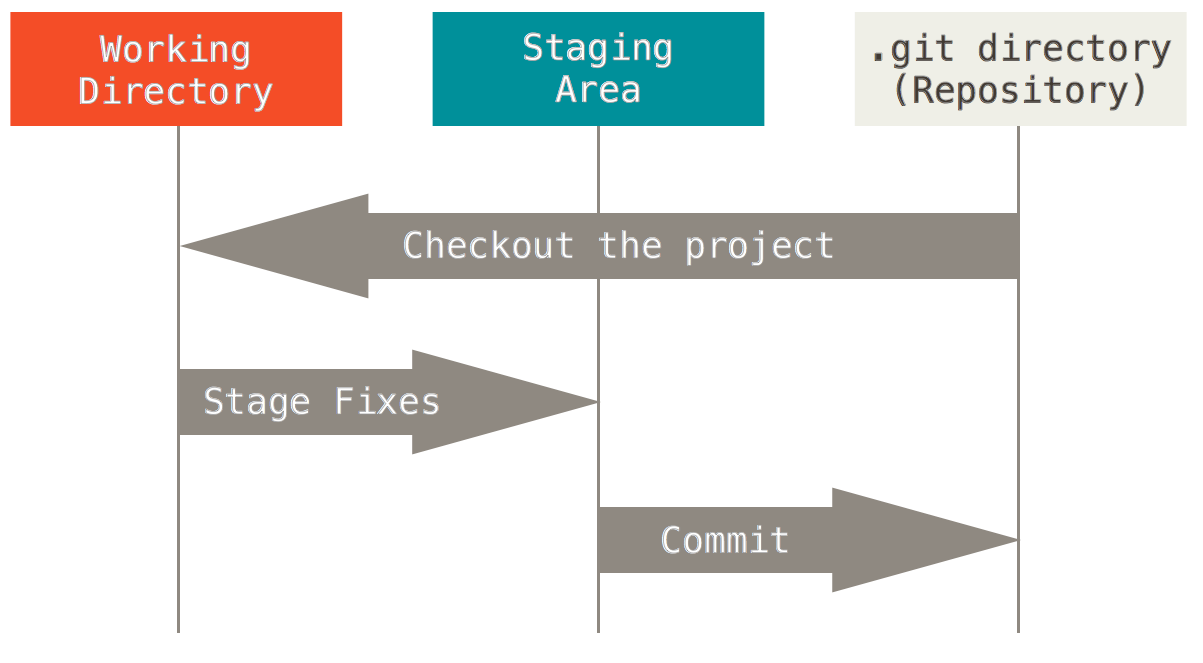
\includegraphics[width=0.9\textwidth]{../img/three_states.png}
    \end{figure}
    % TODO add reference
    % http://www.git-scm.com/book/en/v2/book/01-introduction/images/areas.png
\end{frame}

\begin{frame}
    \frametitle{Lifecycle of our files}
    \begin{figure}[b]{\textwidth}
        \centering
            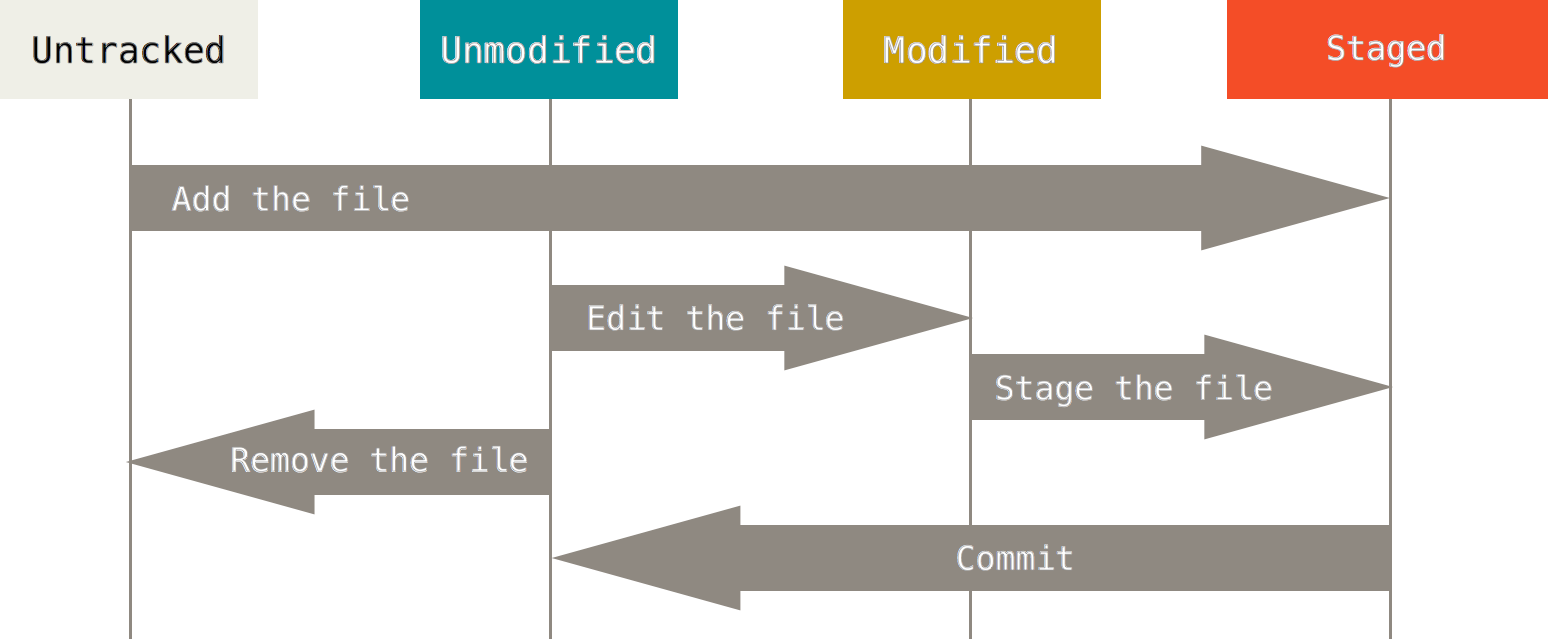
\includegraphics[width=\textwidth]{../img/file_lifecycle.png}
    \end{figure}
    % TODO add reference
    % http://www.git-scm.com/book/en/v2/Git-Basics-Recording-Changes-to-the-Repository
\end{frame}

\begin{frame}
    \frametitle{remote}
    \begin{figure}
        \begin{subfigure}{\textwidth}
            \centering
            \begin{tikzpicture}
                \tikzstyle{stage} = [ rectangle,
                    draw=black!40,
                    fill=black!20,
                    rounded corners,
                    inner sep=0pt,
                    minimum size=1.0cm,
                    thick ]
                    \node[stage] (remote) [label=right:remote \texttt{origin}] {\url{git.kernel.org/pub/scm/git/git.git}};
                    \node[stage] (working) [below=of remote,label=right:local copy] {\url{~/devel/git/git.git}}
                        edge [<-, bend right=45]  node[right] {\tiny{git pull origin master}} (remote)
                        edge [->, bend left=45] node[left] {\tiny{git push origin master}} (remote);
            \end{tikzpicture}
        \end{subfigure}
        \begin{subfigure}[b]{\textwidth}
            \centering
            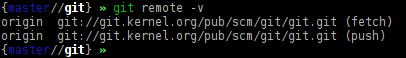
\includegraphics[width=\textwidth]{../img/show_remote.png}
        \end{subfigure}
    \end{figure}
    \texttt{git remote -v} shows where the remote points to.
\end{frame}

\begin{frame}
    \frametitle{adding a remote}
    \begin{figure}
        \begin{subfigure}{\textwidth}
            \centering
            \begin{tikzpicture}
                \tikzstyle{stage} = [ rectangle,
                    draw=black!40,
                    fill=black!20,
                    rounded corners,
                    inner sep=0pt,
                    minimum size=1.0cm,
                    thick ]
                \node[stage] (remote) [label=above:\scriptsize{remote \texttt{origin}}] {kernel.org};
                \node[stage] (remote2) [right=of remote, label=above:\scriptsize{remote \texttt{foo}}] {github.com};
                \node[stage] (working) [below=of remote, xshift=1.25cm, label=right:\scriptsize{local copy}] {localhost}
                    edge [<->, bend left=45] node[auto] {\tiny{git pull origin master}} node[left] {\tiny{git push origin master}} (remote)
                    edge [<->, bend right=45] node[auto] {\tiny{git pull foo master}} node[left] {\tiny{git push foo master}} (remote2);
            \end{tikzpicture}
        \end{subfigure}
        \begin{subfigure}[b]{\textwidth}
            \centering
            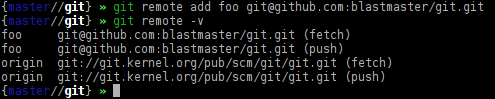
\includegraphics[width=\textwidth]{../img/adding_remote.png}
        \end{subfigure}
    \end{figure}
\end{frame}

\begin{frame}
    \frametitle{Rebasing} %TODO
    \begin{figure}
        \centering
        \begin{tikzpicture}
            \gitDAG[grow right sep = 2em]
            {
                A -- B -- {
                    C,
                    D -- E,
                }
            };
            \gittag
            [v0p1]
            {v0.1}
            {above=of A}
            {A}
            \gitremotebranch
            [origmaster]
            {origin/master}
            {above=of C}
            {C}
            \gitbranch
            {master}
            {above=of E}
            {E}
            \gitHEAD
            {above=of master}
            {master}
        \end{tikzpicture}
    \end{figure}
\end{frame}

\begin{frame}
    \frametitle{Rebasing}
    \begin{figure}
        \centering
        \begin{tikzpicture}
            \gitDAG[grow right sep = 2em] {
                A -- B -- {
                    C -- D' -- E',
                    {[nodes=unreachable] D -- E},
                }
            };
            \gittag
            [v0p1]
            {v0.1}
            {above=of A}
            {A}
            \gitremotebranch
            [origmaster]
            {origin/master}
            {above=of C}
            {C}
            \gitbranch
            {master}
            {above=of E'}
            {E'}
            \gitHEAD
            {above=of master}
            {master}
            \gitblob
            {above=of B}
            {master}
            \SAandWT
            \toSAorWT
            {E}
            {stagingarea}
        \end{tikzpicture}
    \end{figure}
\end{frame}

\begin{frame}
    \frametitle{Tags}
    Tags are like bookmarks on commits.
    \begin{figure}
        \begin{subfigure}[b]{\textwidth}
            \centering
            \begin{tikzpicture}
                \gitDAG[grow right sep = 2em]
                {
                    A -- B -- C
                };
                \gitbranch
                {master}
                {above=of C}
                {C}
                \gitHEAD
                {above=of master}
                {master}
            \end{tikzpicture}
            \subcaption{\texttt{git tag -a v0.1 A}}
        \end{subfigure}
    \end{figure}
\end{frame}

\begin{frame}
    \frametitle{tags}
    \begin{figure}
        \begin{subfigure}[b]{\textwidth}
            \centering
            \begin{tikzpicture}
                \gitDAG[grow right sep = 2em]
                {
                    A -- B -- C
                };
                \gitbranch
                {master}
                {above=of C}
                {C}
                \gittag
                [v0p1]
                {v0.1}
                {above=of A}
                {A}
                \gitHEAD
                {above=of master}
                {master}
            \end{tikzpicture}
            \subcaption{our brand new tag!}
        \end{subfigure}
    \end{figure}
\end{frame}

% demonstrate merging of two branches
\begin{frame}
    \frametitle{merging}
    \begin{figure}
        \begin{subfigure}[b]{\textwidth}
            \centering
            \begin{tikzpicture}
                \gitDAG[grow right sep = 2em]
                {
                    A -- B -- {
                        C,
                        D -- E,
                    }
                };
                \gitbranch
                {master}
                {above=of C}
                {C}
                \gitbranch
                {feature X}
                {above=of E}
                {E}
                \gitHEAD
                {above=of feature X}
                {feature X}
            \end{tikzpicture}
            \subcaption{Before\ldots}
        \end{subfigure}
    \end{figure}
\end{frame}

\begin{frame}
    \frametitle{merging}
    \begin{figure}
        \begin{subfigure}[b]{\textwidth}
            \centering
            \begin{tikzpicture}
                \gitDAG[grow right sep = 2em]
                {
                    A -- B -- {
                        C -- E',
                        {D -- E -- E'},
                    }
                };
                \gitbranch
                {master}
                {above=of E'}
                {E'}
                \gitbranch
                {feature X}
                {below=of E}
                {E}
                \gitHEAD
                {above=of master}
                {master}
            \end{tikzpicture}
            \subcaption{after: \texttt{git merge feature X}}
        \end{subfigure}
    \end{figure}
\end{frame}


